\section{Fold passage and the local sensitivity coefficient}
\label{sec:fold-passage}

This section realizes the Fredholm functional in the polynomial fast--slow
network.  The computation is performed on an invariant graph of compatible
RFDE histories and gives controlled derivatives of a finite-interval
matching function.  This local conclusion is unconditional within the model
assumptions.  Its later identification with a heteroclinic-connection
parameter requires the separate hypotheses in
\cref{sec:heteroclinic-connection}.

\subsection{A locally invariant manifold near the fold}

Set
\[
 s=\delta t,\qquad
 w=\frac23-\delta^2Y,\qquad
 v=\mathbf1+\delta\mathbf1X
       +\delta^2\{z_{2,N}X^2+h\},
 \qquad h\in E_N,
\]
where \(z_{2,N}\) is defined in \cref{eq:rw-fold-center}.
Put
\[
 Z_N(X,h)=z_{2,N}X^2+h.
\]
The singular planar field and its distinguished complete orbit are
\begin{equation}
 q_0(X,Y)=(Y-\alpha X^2,-X),
 \qquad
 \gamma_0(s)=\left(-\frac{s}{2\alpha},
                    \frac{s^2-2}{4\alpha}\right).
 \label{eq:fold-singular-orbit}
\end{equation}
The function
\begin{equation}
 \mathscr H_\alpha(X,Y)
 =\frac12e^{-2\alpha Y}
   \left(\alpha Y-\alpha^2X^2+\frac12\right)
 \label{eq:fold-first-integral}
\end{equation}
is a first integral of \(q_0\), and
\(\nabla\mathscr H_\alpha(\gamma_0(s))
 =(\alpha e/2)e^{-s^2/2}(s,1)^T\).
In these coordinates the transverse singular graph is \(h=0\).  For a
fold-time history \(\phi\), write
\[
 \mathcal L_{N,\eta}[\phi](s)
 =\sum_{k=0}^m(B_{k,N}+\Delta B_{k,N})
       \{\phi(s)-\phi(s-\theta_k)\}.
\]
Direct substitution gives the following identities; there is no Taylor
remainder in this change of variables:
\begin{subequations}\label{eq:fold-exact-system}
\begin{align}
 X'={}&Y-\alpha X^2\notag\\
 &+\delta\left[-2X\pi_N^T\diag(c_N)Z_N
          -\frac\beta3X^3
          +K\pi_N^T\mathcal L_{N,\eta}[\mathbf1X]\right]\notag\\
 &+\delta^2\left[-\pi_N^T\diag(c_N)Z_N^{\circ2}
          +K\pi_N^T\mathcal L_{N,\eta}[Z_N]\right]
 -\delta^3\beta X\pi_N^TZ_N^{\circ2}
 -\frac{\delta^4\beta}{3}\pi_N^TZ_N^{\circ3},
                                                        \label{eq:fold-exact-X}\\
 Y'={}&-X+\delta\nu,                                  \label{eq:fold-exact-Y}\\
 \delta h'={}&A_Nh\notag\\
 &+\delta\left\{P_{\perp,N}\left[-2X\diag(c_N)Z_N
               +K\mathcal L_{N,\eta}[\mathbf1X]\right]
               -2z_{2,N}X X'\right\}\notag\\
 &+\delta^2P_{\perp,N}\left[-\diag(c_N)Z_N^{\circ2}
             -\beta X^2Z_N+K\mathcal L_{N,\eta}[Z_N]\right]
 -\delta^3\beta X P_{\perp,N}Z_N^{\circ2}
 -\frac{\delta^4\beta}{3}P_{\perp,N}Z_N^{\circ3}.
                                                        \label{eq:fold-exact-h}
\end{align}
\end{subequations}
The term \(-2z_{2,N}XX'\) differentiates the translation
\(z_{2,N}X^2\).
The identity
\(A_Nz_{2,N}X^2=P_{\perp,N}c_NX^2\) makes \(h=0\) the transverse
singular graph.

The Dobrushin estimate gives
\begin{equation}
 \|e^{A_Nt}\|_{E_N\to E_N}\le e^{-D\gamma t},
 \qquad
 \|A_N^{-1}\|_{E_N\to E_N}\le(D\gamma)^{-1}.
 \label{eq:fold-poisson-bound}
\end{equation}
Together with the product inequality
\begin{equation}
 \|x_1\circ\cdots\circ x_j\|_N
 \le3\prod_{\ell=1}^j\|x_\ell\|_N,
 \label{eq:fold-product-bound}
\end{equation}
this makes every multilinear bound below independent of \(N\).

Fix \(C_0>0\) and \(p_0>4\), put
\(S_\delta=\sqrt{2p_0\log(1/\delta)}\), and define
\begin{equation*}
 \mathcal U_\delta(C_0)
 =\{\gamma_0(s)+\xi:|s|\le S_\delta+\theta_m,
                         |\xi|\le C_0\delta\}.
\end{equation*}
The extra \(\theta_m\) is the history buffer for the delay translations in
fold time.

We use the standard solution-manifold formulation for smooth RFDEs.  For a
fold-time equation
\(x'=\mathcal F_v(\phi,\omega)\),
\(w'=\mathcal F_w(\phi,\omega)\), define
\begin{equation}
 \begin{split}
 \mathcal M^2(\mathcal F)=\{(\phi,\omega)\in
 C^2([-\theta_m,0];\mathbb R^N)\times\mathbb R:\ {}
 &\phi'(0)=\mathcal F_v(\phi,\omega),\\
 &\phi''(0)=D\mathcal F_v(\phi,\omega)
       [\phi',\mathcal F_w(\phi,\omega)]\}.
 \end{split}                                      \label{eq:C2-solution-manifold}
\end{equation}
Thus elements of \(\mathcal M^2(\mathcal F)\) satisfy the two compatibility
conditions needed for a \(C^2\) solution across the current time.  For a
regular transverse section \(\Sigma\) in the current-state space, write
\begin{equation}
 \mathcal M_\Sigma^2(\mathcal F)
 =\{\Phi\in\mathcal M^2(\mathcal F):
       \operatorname{ev}_0\Phi\in\Sigma\},
 \qquad \operatorname{ev}_0(\phi,\omega)=(\phi(0),\omega).
 \label{eq:C2-solution-manifold-section}
\end{equation}

\begin{proposition}[Locally invariant manifold near the fold]
\label[proposition]{prop:fold-invariant-histories}
Assume \eqref{eq:rw-markov-assumptions}--\eqref{eq:rw-base-layer-bound}.
Fix a compact interval
\(I_\nu\) and \(\eta_*>0\).  Uniformly for \(\nu\in I_\nu\) and
\(\norm{\eta}_{\mathcal T_N}\le\eta_*\), and for all sufficiently small
\(\delta\), there is a two-dimensional locally invariant manifold in the
RFDE phase space, represented over \(\mathcal U_\delta(C_0)\) by the graph
\[
 h=H_{N,\delta,\nu,\eta}(X,Y).
\]
Let \(Q_{N,\delta,\nu,\eta}\) be its reduced vector field and
\(\Phi_Q^s\) its flow.  In fold coordinates the corresponding phase-space
embedding is
\begin{equation}
 \begin{split}
 \iota_{N,\delta,\nu,\eta}:\mathcal U_\delta(C_0)
   &\longrightarrow \mathcal M^2(\mathcal F_{N,\delta,\nu,\eta}^{\rm loc}),\\
 \iota_{N,\delta,\nu,\eta}(u)(\theta)
   &=\bigl(\Phi_Q^\theta u,
      H_{N,\delta,\nu,\eta}(\Phi_Q^\theta u)\bigr),
      \qquad -\theta_m\le\theta\le0,
 \end{split}                                      \label{eq:fold-phase-space-embedding}
\end{equation}
followed by the inverse fold-coordinate change.  Here
\(\mathcal F^{\rm loc}\) is the cutoff RFDE used in the construction.  It
coincides with the original RFDE whenever the orbit and its delayed histories
remain in \(\mathcal U_\delta(C_0)\) and its delay enlargement.  The map
\(\iota_{N,\delta,\nu,\eta}\) is injective, and evaluation at \(\theta=0\),
followed by projection onto \((X,Y)\), is its left inverse.
On \(\gamma_0([-S_\delta,S_\delta])\) it satisfies
\[
 \|H_{N,\delta,\nu,\eta}(\gamma_0(s)+\xi)\|_N
 \le C\delta e^{c|s|}\langle s\rangle^M,
 \qquad |\xi|\le C_0\delta,
\]
and its reduced field has the expansion
\begin{equation}
 Q_{N,\delta,\nu,\eta}
 =q_0+\delta q_{1,N}+\delta^2q_{2,N}
       +\delta^3\mathcal R_{3,N}.                   \label{eq:fold-reduced-expansion}
\end{equation}
For \(0\le a\le3\) and \(0\le i,j\le2\), the derivatives
\(D_{X,Y}^a\partial_\nu^iD_\eta^jH\) and the corresponding derivatives of
the reduced field obey a common bound
\[
 C e^{c|s|}\langle s\rangle^M
\]
on \(\mathcal U_\delta(C_0)\).  Here \(D_\eta^j\) is the symmetric
Fr\'echet derivative in the norm of
\cref{eq:rw-structural-parameter-norm}.  In
particular, \(D_\eta q_{1,N}=0\).  Every embedded history whose orbit and
delay translates remain in the unchanged region is therefore an actual
history of the original RFDE.
\end{proposition}

\begin{proof}
The unknowns are both the graph \(H\) and its planar vector field \(Q\):
the delayed states on the graph are determined by the past flow of \(Q\).
Use the coordinates \(u=(\chi,d)\) from
\cref{eq:supp-fold-coordinates} and a smooth complete extension
\(q_{0,\delta}\) of the singular field.  The cutoffs are fixed independently
of \((\nu,\eta)\).  In these coordinates the extended exact equations read
\[
 u'=q_{0,\delta}(u)+\delta F_{N,\delta},\qquad
 \delta h'=A_Nh+\delta G_{N,\delta},
\]
where \(F_{N,\delta}\) and \(G_{N,\delta}\) are the cutoff versions of the
polynomial terms in \cref{eq:fold-exact-system}.  For a candidate pair
\((Q,H)\), let \(\Phi_Q\) be its complete planar flow and form the finite
tuple
\[
 \mathcal E_{Q,H}(u)=
 \bigl((u,H(u)),\,
       (\Phi_Q^{-\theta_k}u,H(\Phi_Q^{-\theta_k}u))_{k=0}^m\bigr).
\]
The two fixed-point equations are
\begin{align*}
 Q(u)&=q_{0,\delta}(u)+\delta F_{N,\delta}
                (\mathcal E_{Q,H}(u);\delta,\nu,\eta),\\
 H(u)&=\delta\int_0^\infty e^{A_Nr}G_{N,\delta}
       (\mathcal E_{Q,H}(\Phi_Q^{-\delta r}u);\delta,\nu,\eta)\,dr.
\end{align*}
The first equation enforces the collective RFDE on every embedded history;
the second is the stable variation-of-constants equation.  Solving them
together, then undoing the coordinate change, produces the required
invariant manifold.  By \cref{eq:fold-poisson-bound}, their Lipschitz factor is
bounded by
\[
 C\delta P(S_\delta)e^{cS_\delta}
 \int_0^\infty(1+r^M)e^{-D\gamma r/2}\,dr=o(1).
\]
The same estimate applied successively to the finite list of state and
parameter derivatives gives \cref{eq:fold-reduced-expansion}.  Splitting the
stable convolution at \(L\log(1/\delta)\) gives the stated pointwise bounds.
The construction, including the mixed-derivative induction and the exact
history reconstruction, is given in
\cref{subsec:invariant-history-details}.  The auxiliary cutoff used there is
fixed independently of \((\nu,\eta)\) and agrees with the original RFDE on
\(\mathcal U_\delta(C_0)\) and its delay enlargement.
\end{proof}

\subsection{The one-dimensional Fredholm obstruction}

Linearization of \(q_0\) along \(\gamma_0\) gives
\begin{equation}
 L_0(U,V)=(U'-sU-V,V'+U).                            \label{eq:fold-linear-operator}
\end{equation}
The phase condition is \(U(0)=0\).  By
\cref{lem:fredholm-collective-cokernel}, its range has codimension one and is
annihilated by the Gaussian functional in
\cref{eq:fredholm-gaussian-cokernel}; in particular
\(\ell_0(0,1)=\sqrt{2\pi}\).

\subsection{From the delay moment to the collective equation}

The auxiliary parameter \(\rho\) used in the graph construction in
\cref{subsec:invariant-history-details} gives the Taylor expansion
\begin{equation}
 H_{N,\rho,\nu,\eta}
 =\rho H_{1,N,\nu,\eta}+O(\rho^2),
 \qquad
 H_{1,N,\nu,\eta}
 =\left.\partial_\rho H_{N,\rho,\nu,\eta}\right|_{\rho=0},
 \label{eq:fold-first-graph-coefficient}
\end{equation}
in the weighted \(C^3\) norm used for the invariant graph.  Setting
\(\rho=\delta\) recovers the graph of the RFDE.

Let \(R=(R_0,\ldots,R_m)\in\mathcal T_N\) be an admissible
perturbation direction and differentiate the
first graph coefficient with respect to \(\eta\) at \(\eta=0\), in the
direction \(R\), along \(\gamma_0\).  Since
\[
 X_0(s)-X_0(s-\theta_k)=-\frac{\theta_k}{2\alpha},
\]
the transverse equation is
\[
 A_N\left.D_\eta H_{1,N}[R]\right|_{\eta=0}
       -\frac{K}{2\alpha}P_{\perp,N}
       \sum_{k=0}^m\theta_kR_k\mathbf1=0.
\]
Thus
\begin{equation}
 \left.D_\eta H_{1,N}[R]\right|_{\eta=0}
 =A_N^{-1}\mathsf S_NR.                            \label{eq:fold-transverse-variation}
\end{equation}
The row identities \(\pi_N^TR_k=0\) eliminate every direct
delayed-coupling derivative from the collective equation.  More explicitly, write
\(h=\delta H_{1,N}+O(\delta^2)\) on the invariant graph.  The only
contribution from this perturbation to the coefficient of \(\delta^2\) in the first
collective equation is then
\begin{equation*}
 -2X\pi_N^T\diag(c_N)
      \left.D_\eta H_{1,N}[R]\right|_{\eta=0};
\end{equation*}
the direct derivative of
\(K\pi_N^T\mathcal L_{N,\eta}[Z_N]\) vanishes because
\(\pi_N^TR_k=0\).  Since \(X_0(s)=-s/(2\alpha)\),
\cref{eq:fold-transverse-variation,eq:rw-return-functional} give
\begin{equation}
 \left.D_\eta q_{2,N}(\gamma_0(s),\nu,\eta)[R]\right|_{\eta=0}
   =(-\Lambda_N(R)s,0).                             \label{eq:fold-return-source}
\end{equation}
Pairing with \cref{eq:fredholm-gaussian-cokernel} yields
\begin{equation}
 \left.\ell_0\!\left(D_\eta q_{2,N}[R]\right)\right|_{\eta=0}
 =-\sqrt{2\pi}\Lambda_N(R).                        \label{eq:fold-return-pairing}
\end{equation}
This is the concrete realization of the Fredholm expression in
\cref{thm:fredholm-reduction}.  The cancellation takes place
before the delay moment is formed; hence
\cref{eq:fold-return-source} is an identity for the derivatives of the graph
representing the locally invariant manifold, not a current-state formal
expansion.

The order-\(\delta\) collective coefficient is equally explicit.  Along
\(\gamma_0\),
\begin{equation*}
 q_{1,N}(s)
 =\left(\frac{\kappa_N}{8\alpha^3}s^3+C_N,\,\nu\right),
 \qquad
 C_N=-\frac{K}{2\alpha}\pi_N^T
           \left(\sum_{k=0}^m\theta_kB_{k,N}\right)\mathbf1.
\end{equation*}
The constant \(C_N\) has zero pairing with the odd Gaussian factor in
\cref{eq:fredholm-gaussian-cokernel}.  With
\[
 \kappa_N=\frac\beta3
   +2\pi_N^T\diag(c_N)A_N^{-1}P_{\perp,N}c_N,
 \qquad
 \nu_{0,N}=-\frac{3\kappa_N}{8\alpha^3},
\]
and
\(\int_{\mathbb R}s^4e^{-s^2/2}\,\dd s=3\sqrt{2\pi}\), Gaussian
integration gives
\begin{equation}
 \ell_0(q_{1,N})=\sqrt{2\pi}(\nu-\nu_{0,N}).        \label{eq:fold-parameter-pairing}
\end{equation}

\subsection{A finite-interval matching function}

Put \(S=S_\delta\), choose a fixed buffer \(B>2\Theta_*+2\), and set
\(R=S+B\).  Extend the reduced field to \(\widetilde Q\) so that it equals
the invariant-manifold field on the normal strip containing the fold traces
and their delay translates, and equals \(q_0\) near \(\gamma_0(\pm R)\).
The extension operator and cutoffs are fixed independently of \((\nu,\eta)\).
Let \(z^a:[-R,0]\to\mathbb R^2\) and
\(z^r:[0,R]\to\mathbb R^2\) solve the two reduced boundary-value problems
\begin{equation}
 \begin{gathered}
 (z^a)'=\widetilde Q_{N,\delta,\nu,\eta}(z^a),
 \quad (z^r)'=\widetilde Q_{N,\delta,\nu,\eta}(z^r),\\
 X^a(0)=X^r(0)=0,
 \qquad
 \mathscr H_\alpha(z^a(-R))
  =\mathscr H_\alpha(z^r(R))=0.
 \end{gathered}                                    \label{eq:finite-trace-BVP}
\end{equation}
The solutions are unique in a fixed weighted neighborhood
\[
 \sup_{s\in J_\sigma}e^{-c|s|}\langle s\rangle^{-M}
       |z^\sigma(s)-\gamma_0(s)|\le C\delta,
 \qquad J_a=[-R,0],\quad J_r=[0,R].
\]
Their construction and the uniform inverse estimates are given in
Appendix~A.  The scalar matching function is
\begin{equation}
 D_N^{\rm fin}
 =\frac{2}{\alpha e}
   \{\mathscr H_\alpha(z^a(0))-\mathscr H_\alpha(z^r(0))\}.
 \label{eq:finite-matching-definition}
\end{equation}
The traces are exact histories of the original RFDE on the interval where
they and their delayed histories remain in the unchanged region.  Outside that
interval, their auxiliary completion serves only to close the two finite
boundary-value problems.

\begin{proof}[Proof of \cref{thm:rw-local-fold-matching}]
Differentiate the first integral along the attracting and repelling traces
and integrate from their endpoints to the phase section.  The leading terms
are exactly \cref{eq:fold-parameter-pairing,eq:fold-return-pairing}.  The
remaining terms consist of the omitted Gaussian tails, the moving traces,
the graph remainder in \cref{eq:fold-reduced-expansion}, and the fixed
finite-interval boundary conditions.  The graph and trace inverse bounds give
\[
 Ce^{-S_\delta^2/2+cS_\delta}\langle S_\delta\rangle^M
   =C\delta^{p_0-o(1)}=o(\delta^4)
\]
for the tails, while the other first-derivative remainders have the orders
shown in \cref{eq:finite-comparison-level,eq:finite-comparison-structural}.
The exact decomposition and all mixed estimates are proved in
\cref{prop:finite-gap-bridge}.  Combining them with the two Gaussian
pairings proves the three matching estimates.

The uniform bounds on \(A_N^{-1}\) and \(c_N\) bound \(\nu_{0,N}\), so
\(I_\nu\) can be chosen with a common positive buffer around all centers.
Fix \(c_0\) smaller than this buffer.  At
\(\nu=\nu_{0,N}\pm c_0\), the leading terms in
\cref{eq:finite-comparison-level} have opposite signs for small \(\delta\).
Moreover, \cref{eq:finite-comparison-slope} gives
\(\partial_\nu D_N^{\rm fin}\ge\delta\sqrt{2\pi}/2\) on the window.
There is therefore exactly one zero \(\nu_N^{\rm fin}\), and the
Banach implicit-function theorem makes it \(C^1\) in \(\eta\).  On its graph,
\[
 D_\eta\mu_N^{\rm fin}
 =-\delta^2\frac{D_\eta D_N^{\rm fin}}{\partial_\nu D_N^{\rm fin}}
 =\delta^3\Lambda_N+
       O(\delta^4+\delta^3\norm{\eta}_{\mathcal T_N}).
\]
This proves \cref{eq:rw-local-root-sensitivity}; integrating along
\(t\mapsto t\eta\), \(0\le t\le1\), gives
\cref{eq:rw-local-root-increment}.
\end{proof}

\subsection{Prescribed-history numerical diagnostics}

For the three-node example in the introduction, set
\(\sigma=1/2\), \(\beta=3\), \(D=1\), \(K=2\),
\((\theta_0,\theta_1)=(1,2)\), and \(B_0=B_1=P/2\).
Prescribe \((X,Y,h)=(-s/2,(s^2-2)/4,0)\) on \([-S-2,-S]\), and integrate
\cref{eq:fold-exact-system} to \(S\).  Let
\(\widehat\nu_{\rm sec}(\delta,\zeta;S)\) be a zero of the outgoing
condition \(\widehat E_S=Y(S)-X(S)^2+1/2\).  With \(\zeta_*=0.04\), define
\begin{equation}
 \widehat q(\delta,S)=
 \frac{\widehat\nu_{\rm sec}(\delta,\zeta_*;S)
       -\widehat\nu_{\rm sec}(\delta,-\zeta_*;S)}{2\zeta_*\delta}.
 \label{eq:numerical-section-quotient}
\end{equation}
The incoming history is prescribed and is not obtained from the invariant
history graph; hence these zeros are defined by a different problem from
the finite matching zeros \(\nu_N^{\rm fin}\).  Their purpose is to test whether the sign and scale of
the analytically computed response can be observed in a direct RFDE
integration.

Figure~\ref{fig:three-node-finite-section} shows the displacement of the
section zeros and the quotient compared with \(\Lambda_3=-1/3\).  The
diagonal schedule in panel~\textbf{(b)} varies both \(\delta\) and \(S\).
Table~\ref{tab:window-grid} separates these effects.  At \(S=3.5\) and
\(S=4\), the displayed decreasing values of \(\delta\) improve agreement
with \(-1/3\).  At \(S=3\), the quotient crosses this value and then moves
away; dependence on \(S\) is also not uniformly monotone.  The results retain
finite-history and finite-section bias and do not establish an asymptotic
error bound for the invariant-manifold matching problem.

\begin{table}[tb]
\centering
\caption{Prescribed-history quotient \(\widehat q(\delta,S)\) on a
rectangular parameter grid.  The analytic reference is \(\Lambda_3=-1/3\).
The perturbation step is fixed at \(\zeta_*=0.04\).}
\label{tab:window-grid}
\begin{tabular}{@{}rrrr@{}}
\toprule
\(\delta\) & \(S=3\) & \(S=3.5\) & \(S=4\)\\
\midrule
0.05 & -0.340829 & -0.344640 & -0.337948\\
0.02 & -0.330866 & -0.336188 & -0.334582\\
0.01 & -0.327618 & -0.333655 & -0.333703\\
\bottomrule
\end{tabular}
\end{table}

The computations use the method of steps with the Radau solver, relative and
absolute tolerances \(2\times10^{-9}\) and \(2\times10^{-11}\), maximum
step \(0.08\), and Brent root tolerances \(2\times10^{-10}\).
At \((\delta,S)=(0.05,4),(0.01,3),(0.01,3.5)\), tightening these to
\(5\times10^{-10}\), \(5\times10^{-12}\), \(0.04\), and
\(10^{-11}\), respectively, changes the quotient by less than
\(1.5\times10^{-8}\).  This is a numerical refinement check, not a rigorous
enclosure.  The source archive records the parameters, source hashes,
software versions, and all computed roots.

Panel~\textbf{(c)} uses the growing family in \cref{prop:rw-growing-families}
with \(\rho=1\), \((\delta,S)=(0.02,3.5)\), and the same remaining
parameters.  The values at \(N=3,5,9,17,33\) stay within \(0.008\) of
\(\Lambda_N=-1/2\), illustrating persistence of the response under uniform
mixing.

\begin{figure}[p]
\centering
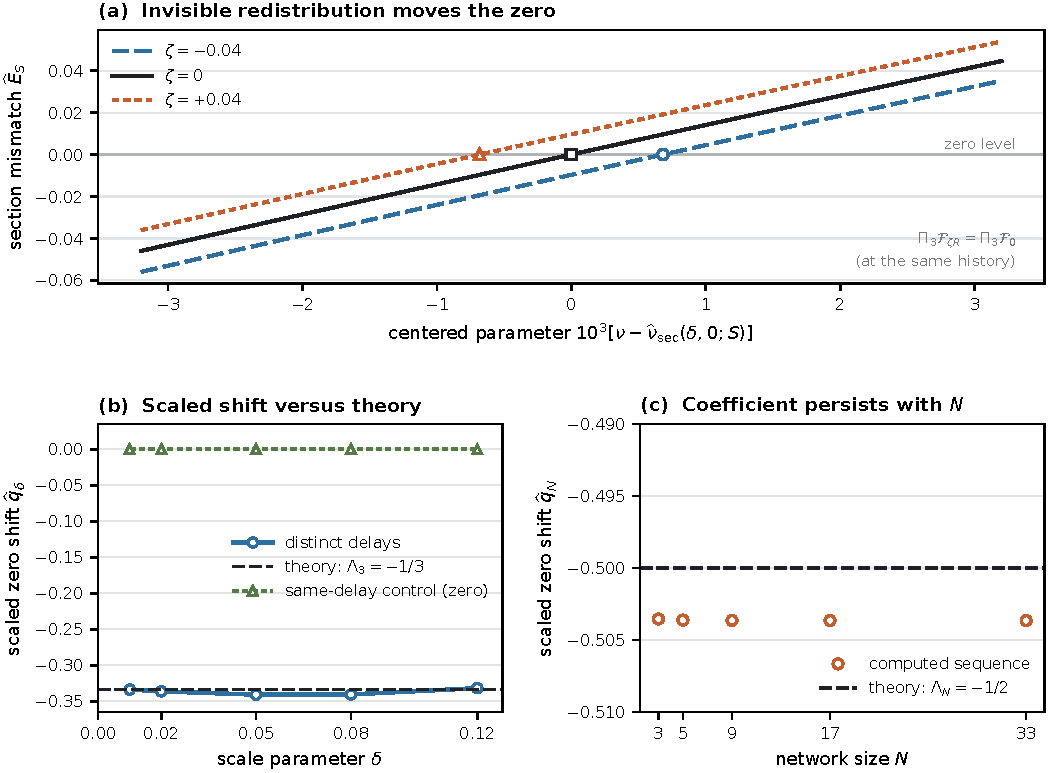
\includegraphics[width=\textwidth]{figures/three-node-finite-section.pdf}
\caption{Prescribed-history section diagnostics for the local Fredholm
coefficient, with parameters from \cref{eq:numerical-section-quotient} and
its preceding paragraph.  \textbf{(a)} The marked zeros of
\(\widehat E_S=Y(S)-X(S)^2+1/2\) shift under opposite perturbations of the two
delay layers, while the projected vector field is unchanged at each fixed
history; \((\delta,S)=(0.05,3)\).
\textbf{(b)} The computed quotient is compared with \(\Lambda_3=-1/3\) along
\((\delta,S)=(0.12,2.5),(0.08,2.75),(0.05,3),(0.02,3.5),(0.01,4)\).
Combining the perturbation layers at one delay makes their contribution
cancel exactly (green triangles).
\textbf{(c)} The growing family at \(N=3,5,9,17,33\) has computed quotients
close to its common coefficient \(\Lambda_N=-1/2\).  Symbols and curves are
numerical; dashed reference coefficients and the cancellation identity are
analytic.  This calculation is not \(D_N^{\rm fin}\) and does not compute a
heteroclinic connection or a maximal canard.}
\label{fig:three-node-finite-section}
\end{figure}

